\documentclass[11pt]{article}
\usepackage[margin=1in]{geometry}
\usepackage[T1]{fontenc}
\usepackage{lmodern}
\usepackage{microtype}
\usepackage{amsmath,amssymb}
\emergencystretch=2em
\usepackage{booktabs}
\usepackage{graphicx}
\usepackage{xcolor}
\usepackage[hidelinks]{hyperref}
\usepackage{enumitem}
\setlist{nosep,leftmargin=1.4em}

\newcommand{\entry}[2]{\subsection*{#1\hfill{\normalfont\small\texttt{#2}}}}
\newcommand{\src}[1]{{\small\color{black!60}Source: \texttt{#1}}}

\title{\textbf{Spectre: Experiment Log}\\[0.3em]\large Spectrum to structure retrieval on MassSpecGym under an evaluator that cannot be gamed}
\author{Spectre team\\\small SF AI Research Hackathon}
\date{November 15, 2026}

\begin{document}
\maketitle

\begin{abstract}
\noindent
This is the running lab notebook for Spectre. Each entry records what was run, on what data, and what came out, with
the log file that holds the raw numbers. The task is MassSpecGym retrieval with formula candidates~\cite{msg}: given
an MS/MS spectrum, rank up to 256 candidate molecules that share its formula. Two findings so far. First, the raw
candidate lists put the true molecule first for every one of 8{,}000 val and test spectra, so an unshuffled
benchmark can be solved without reading a spectrum. Second, adding a neutral loss channel to a fingerprint MLP gives a
gain that clears the seed noise band on the two seeds scored so far and does not survive either canary.
Numbers marked \emph{partial} come from runs that were still in progress when this entry was written.
\end{abstract}

\section*{Setup}

\textbf{Data.} HuggingFace \texttt{roman-bushuiev/MassSpecGym}, file \texttt{MassSpecGym.tsv}, with the official
MCES disjoint \texttt{fold} column. Candidates come from the formula candidate file
(\texttt{MassSpecGym\_retrieval\_\allowbreak candidates\_formula.json}), keyed by query SMILES.

\textbf{Splits.} All 194{,}119 train spectra. Val and test are fixed random subsets of 4{,}000 spectra each
(\texttt{pandas.sample}, seed 0) drawn from folds of 19{,}429 and 17{,}556 spectra.

\textbf{Metrics.} hit@$k$ for $k \in \{1,5,20\}$ and MRR@20. The Referee decides on MRR@20. A prediction matches when
the SMILES string or the first 14 characters of the InChIKey agree with the label. Random ranking has expected hit@1
\begin{equation*}
  \mathbb{E}[\text{hit@1}] = \frac{1}{N}\sum_{i=1}^{N} \frac{1}{n_i},
\end{equation*}
where $n_i$ is the number of candidates for spectrum $i$.

\textbf{Fingerprints.} Morgan radius 2, 2048 bits, RDKit 2024.9.6, stored bit packed (256 bytes per candidate).

\section*{Entries}

\entry{E1. Data preparation and a leak in the candidate lists}{06:18 PT}

Built the train, val and test parquet files and fingerprinted every candidate of the 8{,}000 val and test spectra
(599{,}629 unique SMILES, all parsed by RDKit, none failed). Every val and test spectrum has its true molecule among its
candidates.

While building the files we recorded where the true molecule sits in each original candidate list.
It is at index 0 in all of them (Table~\ref{tab:leak}). Any model that returns the list unchanged scores hit@1 of 1.0.
We now shuffle every list with a per spectrum RNG seeded by \texttt{(0, crc32(id))}, and shuffle the fingerprint rows
with it. After the shuffle the true molecule is first about as often as chance predicts.

\begin{table}[h]
\centering
\begin{tabular}{lrr}
\toprule
 & Val & Test \\
\midrule
Spectra & 4{,}000 & 4{,}000 \\
Candidates per spectrum, mean (min, max) & 159.8 (1, 256) & 165.9 (1, 256) \\
True molecule in candidate list & 100\% & 100\% \\
True molecule at index 0, original order & \textbf{4{,}000 of 4{,}000} & \textbf{4{,}000 of 4{,}000} \\
True molecule at index 0, after shuffle & 4.2\% & 3.1\% \\
Expected random hit@1 & 3.77\% & 3.00\% \\
\bottomrule
\end{tabular}
\caption{Candidate list statistics. The original order leaks the label.}
\label{tab:leak}
\end{table}
\src{runs/prep.log, bench/prep.py}

\entry{E2. Baseline}{06:30 PT}

\textbf{Model.} Spectrum binned at 0.1\,Da up to 1000\,Da (10{,}000 bins), square root of intensity relative to the base
peak, plus precursor $m/z$ and a one hot adduct. Two hidden layers of 1024 with ReLU and dropout 0.3, output 2048
logits, binary cross entropy against the true fingerprint. AdamW, one cycle schedule, peak learning rate
$10^{-3}$, 25 epochs, batch 512. Candidates are ranked by cosine similarity between the predicted bit probabilities and
each candidate fingerprint, as in CSI:FingerID style retrieval~\cite{csifingerid}.

\textbf{Run.} The first attempt on an A10G was refused because the Modal account had no payment method. We ran the
same code on a 16 core CPU container instead (576\,s training).

\textbf{Result.} Val hit@1 0.1003, hit@5 0.2298, hit@20 0.4195. A random ranking of the same lists scores
0.0395, 0.1175 and 0.2935. The baseline is 2.7 times random at hit@1.

\src{runs/baseline\_seed0\_cpu.log, bench/baseline/model.py}

\entry{E3. Hand written candidate: neutral losses}{06:43 PT}

\textbf{Hypothesis.} Neutral losses, the mass differences between the precursor and each fragment, carry structure
information (loss of water, CO$_2$, ammonia, sugars) that $m/z$ bins capture only indirectly~\cite{neutralloss}. A
model given them explicitly should rank better while still depending on the spectrum.

\textbf{Changes.}
\begin{enumerate}
  \item A second channel of 5{,}000 bins for $\text{precursor } m/z - \text{fragment } m/z$ between 0 and 500\,Da, at
        0.1\,Da, weighted by the same square root intensity as the peak.
  \item The first dense layer replaced by an \texttt{EmbeddingBag} over peak bins with intensity weights. This computes
        the same function as the dense layer on a sparse input and is cheaper, which pays for change 1.
  \item Optionally, a cosine term added to the loss,
        $\mathcal{L} = \text{BCE} + \lambda\,(1 - \cos(\sigma(z), y))$, since ranking uses cosine.
\end{enumerate}
Every spectrum derived input is multiplied by peak intensity, so zeroing intensities removes all of it.

\textbf{Sweep.} Five variants, seed 0, run in parallel on 16 core CPU containers. A wider network
(2048 hidden, 30 epochs) ran at about 77\,s per epoch, which exceeds the 15 minute budget, and was stopped.

\begin{table}[h]
\centering
\begin{tabular}{lcccr}
\toprule
Model & hit@1 & hit@5 & hit@20 & Train (s) \\
\midrule
Random ranking & 0.0395 & 0.1175 & 0.2935 & \\
Baseline & 0.1003 & 0.2298 & 0.4195 & 576 \\
Sparse first layer & 0.1070 & 0.2295 & 0.4250 & 520 \\
Sparse, cosine loss & 0.1078 & 0.2295 & 0.4300 & 389 \\
Sparse, neutral losses, cosine loss & 0.1130 & \textbf{0.2425} & 0.4278 & 684 \\
\textbf{Sparse, neutral losses} (kept) & \textbf{0.1145} & 0.2378 & 0.4285 & 456 \\
\bottomrule
\end{tabular}
\caption{Seed 0 val sweep on CPU. Single seed numbers.}
\label{tab:sweep}
\end{table}

\begin{figure}[h]
\centering
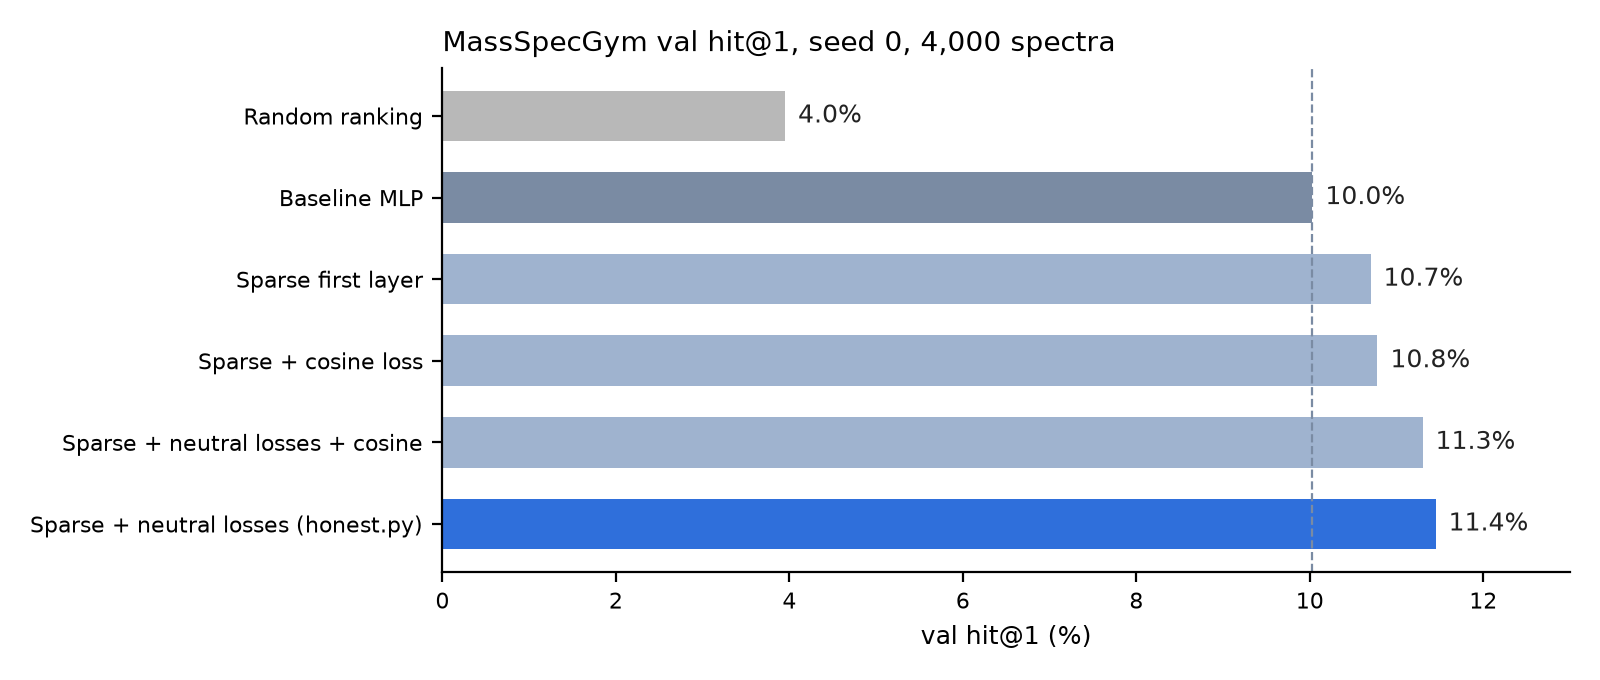
\includegraphics[width=0.85\linewidth]{honest_sweep_hit1.png}
\caption{Val hit@1 for each variant in Table~\ref{tab:sweep}. The dashed line is the baseline.}
\end{figure}

\textbf{Observations.}
\begin{itemize}
  \item The sparse first layer alone computes the same function as the baseline yet scored 0.7 points higher. That
        difference is initialization and seed noise, and it sets the scale for what a single seed can show.
  \item Neutral losses add 0.75 points over the matched sparse run, with or without the cosine term.
  \item The cosine term did not help hit@1 and made training 1.5 times slower, so it is off by default
        (\texttt{COS\_W = 0}).
\end{itemize}
\src{runs/honest\_sweep.log, bench/candidates/honest.py}

\entry{E4. Referee runs on GPU (partial)}{07:26 PT}

The Referee trains each submission in a network isolated GPU sandbox, three seeds on val, then two canaries on seed 0.
The \emph{ablate} canary zeroes every intensity at inference. The \emph{shuffle} canary permutes structures across
training spectra before training. A claim is promoted only if its paired MRR@20 gain has a bootstrap 95\%
CI~\cite{koehn} above zero, exceeds twice the incumbent's seed to seed standard deviation, is positive on every seed,
keeps less than half of itself under each canary, and holds on the hidden test fold.

\begin{table}[h]
\centering
\begin{tabular}{llcccc}
\toprule
Model & Run & MRR@20 & hit@1 & hit@5 & hit@20 \\
\midrule
Baseline & seed 0 & 0.1648 & 0.1013 & 0.2298 & 0.4220 \\
         & seed 1 & 0.1663 & 0.1065 & 0.2260 & 0.4238 \\
         & seed 2 & 0.1616 & 0.0993 & 0.2233 & 0.4228 \\
         & seed 0, ablate & 0.1044 & 0.0522 & 0.1555 & 0.3230 \\
         & seed 0, shuffle & 0.0806 & 0.0393 & 0.1140 & 0.2993 \\
\midrule
Neutral losses & seed 0 & 0.1731 & 0.1128 & 0.2323 & 0.4348 \\
               & seed 2 & 0.1754 & 0.1158 & 0.2372 & 0.4343 \\
               & seed 0, ablate & 0.1059 & 0.0558 & 0.1562 & 0.3150 \\
               & seed 0, shuffle & 0.0839 & 0.0420 & 0.1165 & 0.2895 \\
\midrule
Prior trap & seed 0 & 0.1407 & 0.0823 & 0.1990 & 0.3935 \\
           & seed 2 & 0.1403 & 0.0835 & 0.1898 & 0.3870 \\
\bottomrule
\end{tabular}
\caption{Referee runs on val, GPU sandbox. Seed 1 of the neutral loss model and the remaining prior trap runs had not
finished.}
\label{tab:referee}
\end{table}

\textbf{Noise band.} The baseline's MRR@20 over three seeds has standard deviation 0.0024 (sample std), so the band is
$\pm 0.0048$.

\textbf{Neutral losses versus baseline, paired by spectrum.}
\begin{center}
\begin{tabular}{lcc}
\toprule
 & MRR@20 gain & Bootstrap 95\% CI \\
\midrule
Seed 0 & $+0.0083$ & $[+0.0008,\ +0.0155]$ \\
Seed 2 & $+0.0137$ & $[+0.0071,\ +0.0208]$ \\
\bottomrule
\end{tabular}
\end{center}
Both gains exceed the noise band. Under the ablate canary the gain falls to $+0.0015$, about 14\% of the seed 0
and 2 mean of $+0.0110$. Under the shuffle canary it is $+0.0033$, about 30\%. Both are below the 50\% threshold, so on
the evidence so far the gain comes from reading the spectrum. Seed 1 and the hidden test fold are still pending.

\textbf{Prior trap.} \texttt{bench/redteam/prior.py} adds the cosine to the mean training fingerprint to every
candidate score with weight 1.0. It was planted to produce a fake gain that survives zeroed spectra. At this weight it
\emph{lowers} MRR@20 by 0.021 to 0.024 on both seeds, so the Referee will reject it as noise rather than as a prior. To
demonstrate the PRIOR verdict the trap needs a weight that actually raises val MRR@20.

\textbf{GPU versus CPU.} The same seed 0 code gives hit@1 0.1013 on GPU and 0.1003 on CPU for the baseline, and 0.1128
versus 0.1145 for the neutral loss model. Small differences between devices are
expected, so every comparison in Table~\ref{tab:referee} uses GPU runs only.

\src{runs/referee\_cache.json, runs/seeded.log, bench/referee.py}

\section*{Open items}
\begin{itemize}
  \item Finish seed 1 of the neutral loss model and score the hidden test fold.
  \item Retune the prior trap weight so it yields a real val gain, then confirm the PRIOR verdict.
  \item Score \texttt{noise.py} seed 0 (plain) to complete its verdict.
  \item Log swarm claims and verdicts here as they arrive.
\end{itemize}

\begin{thebibliography}{9}\small
\bibitem{msg} R.~Bushuiev et al. MassSpecGym: A benchmark for the discovery and identification of molecules.
  NeurIPS Datasets and Benchmarks, 2024.
\bibitem{csifingerid} K.~D\"uhrkop et al. Searching molecular structure databases with tandem mass spectra using
  CSI:FingerID. PNAS, 2015.
\bibitem{neutralloss} A.~Aisporna et al. Neutral loss mass spectral data enhances molecular similarity analysis in
  METLIN. JASMS, 2022.
\bibitem{koehn} P.~Koehn. Statistical significance tests for machine translation evaluation. EMNLP, 2004.
\end{thebibliography}

\end{document}
